\chapter{Initial Tool}

\section{Motivation}

The culmination of our research and interviews with founders and investors was the proposal of VCWiz, a three-part platform geared towards helping first-time founders better research, discover, and outreach their optimal seed investors. The focus on seed-stage companies reflected the industry opinion that early-stage venture was an insider's game, where as later rounds of funding were more dependent on quantitative metrics around the companies growth, traction, and success. In the spirit of making venture more accessible and efficient, we chose to focus on first-time founders, who do not necessarily have the connections and tribal knowledge that makes their more experienced counterparts so much more likely to succeed.

We conducted a series of user interviews (N = 21) to determine which aspects of the platform would be most crucial, and what functionality the first version of this application should contain. The interviews were conducted across the spectrum of experience, from first-time student founders to industry veterans, based in New York, Boston, and San Francisco, and working on everything from novel social networks to machine learning-powered drug discovery. We also consulted with several reputable investors at top-tier firms such as First Round Capital and General Catalyst.

We can summarize our user interview feedback into the following three feature buckets.

\subsection{Discovery}

Founders often complain that it is difficult to discover the set of investors that are applicable to their startup. Investors, especially at the seed stage, have a plethora of conditions imposed on the capital they distribute, including restrictions on location, industry, target market size, business model, amount of capital being raised, valuation of the startup, and terms of the deal. Frustratingly, these conditions are rarely published anywhere, meaning it is difficult to query a list of investors to reveal the ones that match your conditions as a founder. This leaves founders resorting to overwhelmingly large databases of investors, or boutique, curated lists which might miss less well-known options for capital.

\subsection{Research}

Once an eligible set of venture firms has been found, the burden on the founder only increases. In addition to figuring out the specific constraints mentioned above, each firm has preferences that may or may not align with the founder's vision for the company. Furthermore, in today's markets, where capital is widely available and there are many similar sources of capital, venture firms are fighting to differentiate themselves to founders, adding another degree of freedom to the ranking function each founder must internally maintain. ``The evidence suggests that VCs' `extra‐financial' value may be more distinctive than their functionally equivalent financial capital''~\cite{doi:10.1111/j.1540-6261.2004.00680.x}, but what exactly the extra-financial value of a firm is can often be difficult to uncover without a meeting or phone call. A vast increase in the number of new seed-stage funds being started further exacerbates the problem: venture research firm CBInsights claims that ``the number of funds closed in 2014 was nearly 100\% more than 2013''~\cite{cbinsights-research-barbell}.

A separate concern from the selection of the venture firm is the selection of the General Partner within the firm. Our data shows that there are an average of 4.68 partners per venture firm, with several other associates and supporting staff on the investment team. Each person often has an area of expertise and a type of company they prefer to consider, as well as a particular way to engaging with the companies they support. However, as before, there is no easy way to tell which parters prefer which industries or business models, making the selection process for founders laborious at best, and arbitrary in the average case.

\subsection{Outreach}

The final major burden for founders who have identified and researched their ideal (seed) investors is to find a way to get connected to each one. It's commonly accepted in the industry that a so-called ``warm introduction'', that is, a direct introduction from someone who personally knows the investor, is the best way to start a conversation with a VC. Indeed, this is corroborated by the data. It has been shown that ``direct ties are strongly and positively related to the probability of investment''~\cite{doi:10.1287/mnsc.48.3.364.7731}, in support of the hypothesis that ``investors are more likely to invest in new ventures when they have a previously established direct tie to the entrepreneur than when they do not''~\cite{doi:10.1287/mnsc.48.3.364.7731}. The further removed a founder is in the global social graph from an investor, the less chance they will be able to get a direct introduction, and the lower the likelihood of investment. However, for many first-time founders, it is simply impossible to get a direct introduction at all. The problem then shifts to finding the best ``intro path'' to a given investor, or barring that, sending the ``cold'' email which maximizes the chance the investor will consider taking a meeting. This process is often ad-hoc and confusing.

\section{Existing Solutions}
\label{vcwiz:existing}

Several solutions exist which solve one or many of the problems discussed above, but there has yet to be a comprehensive solution. As we will discuss later, the threshold at which a product is considered sufficiently feature-complete is very high. Though many of the founders we interviewed used pieces of these solutions, none of them were satisfied with the status quo, and every one thought that the state of existing tools could be improved.

\subsubsection{Crunchbase}

Crunchbase \footnote{https://crunchbase.com} is an online database of companies, their founders, and the investors that back them. It was created ``to be the master record of data on the world’s most innovative companies''~\cite{doi:10.1287/mnsc.48.3.364.7731}, and is largely used as the first place founders go to learn more about a startup's investors. While the database is very comprehensive (and indeed was use to seed the database for VCWiz), it has historically been cumbersome to navigate, and the founders we interviewed found it to be a poor choice for discovery, though an excellent first step for research.

The database offered through the Crunchbase Data Venture Program \footnote{https://about.crunchbase.com/partners/venture-program/} was used to seed the VCWiz investor database.

\subsubsection{AngelList}

AngelList \footnote{https://angel.co} is ``a platform for startups'', which focuses on early-stage companies and investors (both Angels and institutional seed investors). The core platform has social networking, and a directory of startups, their employees, and their early investors, akin to Crunchbase. AngelList's dataset is less comprehensive than Crunchbase's, and narrower in scope. Thus, the founders we interviewed found it less helpful for both research and discovery (though extremely helpful for recruiting employees).

\subsubsection{LinkedIn}

LinkedIn \footnote{https://linkedin.com} is a very popular professional networking platform that founders often use to find mutual connections to investors, so as to solicit introductions. The biggest complaint of founders using LinkedIn for this purpose was that it was not integrated into the rest of their workflow, though this was only expressed in a minority of those surveyed.

\subsubsection{NFX Signal}

Signal \footnote{https://signal.nfx.com} is a platform for founders to find introduction paths to VCs. Founders on Signal grant the application access to their Gmail inboxes, and in return can see the chain of people who comprise the shortest path to any given investor. The graph is built up based solely on email activity, and profile information for investors is self-reported. While this product successfully solves the problem of figuring out which individuals in one's network can provide the introduction to an investor, founders we interviewed often shied away from using it, citing privacy concerns. Signal is operated by NFX Guild, a venture firm, and founders are often unclear about how their email data is being used.

The methodology for displaying investors on Signal \cite{signal-methodolody} was the inspiration for the VCWiz ranking algorithm.

\subsubsection{Streak}

The Streak CRM \footnote{https://www.streak.com} is a popular Gmail extension which embeds a spreadsheet-like customer relationship management (CRM) system in your mailbox. It tracks the progress of conversations, updating itself based on the emails being sent and received by the user. Streak offers a template set of headers and categories for fundraising \footnote{https://www.streak.com/startup-fundraising-management-inside-google-gmail}, which is often used by founders. This means of tracking outreach and progress during a funding round was one of the most popular in the founders we interviewed: there were very few complaints, other than that this setup still requires substantial manual data entry.

The spreadsheet-like interface for tracking conversations with Streak was the inspiration for the conversation tracker in the first version of VCWiz.

\subsubsection{Affinity}

Affinity \footnote{https://affinity.vc} is a modern CRM solution which includes many features that make fundraising easier and more efficient. It is fully automated, with every conversation a founder has by email appearing on the platform, along with pre-filled information about investors and firms. It solves many of the qualms founders have with simpler CRM systems such as Streak, and includes a social graph which suggests introduction paths, as Signal does. The platform solves many of the common complaints around fundraising tooling, though it comes at a premium. Our interviews showed that many founders consider it to be too expensive to use.

\subsubsection{Foundersuite}

Foundersuite \footnote{https://foundersuite.com} is a comprehensive set of tools for fundraising. It is as sophisticated as Affinity, but developed specifically for founders. The CRM component of Foundersuite features a card-based system with manual updating of where each investor is in the fundraising pipeline. The software also includes a pre-populated database of investors which is used to autofill fields, and provide a search tool. Like Affinity, the common complaint with Foundersuite was the cost, and complexity.

The set of features and tools offered by Foundersuite were used as the starting feature set for VCWiz.

\section{Our Tool}
\label{chap3:tool}

The first step towards improving the founder-investor matching process is better tooling for both ends. Since founders are often the individual initiating an interaction, it makes sense to first focus on founders. After reviewing the existing solutions, and the feedback of founders as above, it's clear that there is an opportunity for a product which is sufficiently comprehensive yet much more accessible (with respect to cost and usability).

Fundraising can look very different at different stages of a company's life. While raising a pre-seed or seed round can entail leveraging a network to meet and impress sufficient investors until (at least) on decides to invest, later rounds of funding (e.g. Series A or B) are more predicated on the quantifiable traction of the company. Thus, a lot of the tools above are most impactful for seed-stage founders.

The process of fundraising also looks very different for the subset of founders that are so-called serial entrepreneurs: having raised money from institutional investors in the past means a founder no longer necessarily has the issue of discovering who they should take money from. Furthermore, ``entrepreneurs with a track record of success are much more likely to succeed than first-time entrepreneurs''~\cite{gompers2010performance}. Research on retail businesses shows that indeed, even outside of technology, ``prior business experience increases the longevity of the next business opened''~\cite{doi:10.1086/683820}. Indeed, the investing side of the equation also believes this. Data from the First Round Capital 10 Year Project \cite{first-round-10-years} indicates that ``repeat founders’ initial valuations tended to be over 50\% higher'' than those of first-time founders.

Thus, in order to maximize the impact we have on the equity and efficiency of the founder-investor matching process, we opted to design a tool geared towards first-time founders, who are raising their first (seed) rounds. The tool has discovery, research, and outreach components, borrowing interfaces and functionality from the best of the above-discussed tools. We call our new tool VCWiz. VCWiz went through three iterations, each substantially changing the functionality and interface according to feedback solicited from users. We will first discuss the first iteration of VCWiz.

The components of the solution offered by VCWiz are split into the same categories considered above. We will first discuss the theoretical solutions to be offered by the tool, and then dive into the implementation and lessons learned for the first two iterations. The final version, which is currently live, is described in the next chapter.

The current version of VCWiz can be found at \url{https://vcwiz.co/}.

\subsection{Discovery}

To solve the discovery problem, we identified the several key characteristics which founders look for in a given venture capital firm. These include:

\begin{itemize}
  \item the location of the firm
  \item the industries the firm has invested in
  \item the average check size of the firm
  \item the number of investments a firm makes annually
  \item the companies a firm has invested in
\end{itemize}

The goal of the platform is to let the founder specify their preferences in any of these characteristics, and for the system to recommend relevant investors based on those preferences, and information collected about the founder (the stage, industry, and location, and competitors of their startup).

\subsection{Research}

After surfacing recommendations to the founder, the platform strives to be the single location with all the relevant information about the partners of a given venture firm. The goal is that the founder never has to leave VCWiz (or a site linked from VCWiz) in order to make a decision about an investor. To this end, in addition to the characteristics necessary for discovery, we collect and report several other pieces of information:

\begin{itemize}
  \item The most recent investments of the firm
  \item The most recent investments of a given partner at the firm
  \item The firms that often invest alongside a firm (``co-investors'')
  \item The specific industries that a partner focuses on investing in
  \item The topics a partner often discusses online
  \item Links to online profiles and content created by the firm or a partner
  \item Biographic and demographic information on a partner
\end{itemize}

\subsection{Outreach}

Finally, once a founder has filtered their recommendations using the research tools on the platform, the final job of VCWiz becomes to ensure the founder can begin a conversation with their desired investors. To measure progress on this front, the platform contains a ``conversation tracker'': a CRM which auto-populates the profiles of investors marked as desirable by the founder, and auto-updates as the founder has conversations with those investors. The goal of this CRM is to be as automatic as possible, making assumptions wherever it can.

In addition to simply tracking conversations, VCWiz offers two tools for initiating them. The first is a NFX Signal-style introduction path system, which leverages the social graph of the founder to identify the optimal shortest path to any given investor, if one exists. The second tool is a structured system for automated introductions: the founder can request an introduction to an investor, who gets a consistently-formatted, auto-generated dossier on the startup. The investor then has the choice of accepting or rejecting the introduction request. This system is an experiment to see how structure and consistency can improve the process of cold outreach, and is discussed later.

\section{Tool Iterations}

\subsection{V1}

\subsubsection{Design}

The first step in building the first version of VCWiz was to spent time talking to 21 teams of startup founders, going through well-known accelerators such as Y Combinator\footnote{http://www.ycombinator.com/} (``one of the oldest and top-rated incubator/accelerator programs in the country''~\cite{stross2013launch}). This occurred in June of 2017. The goal was to capture these founders right as they were about to begin raising their seed (initial) rounds of funding. They all identified a need for personalized suggestions of investors. Our initial idea was to collect information from each founder on their ideal investor (characterizing investors and firms with features such as industry, check size, and location), and generate suggestions from a cluster of similar investors (using an item-based k-nearest neighbors model, as in \cite{Stone:2013:EST:2541167.2507882}). With this in hand, we build the first iteration of the VCWiz application.

The first version of VCWiz collected a founder's ideal investor profile (based on the characteristics identified above), as well as basic company information, before taking them to a screen of recommendations. The founder had the option to add any of the recommended investors to a list of ``target investors'' to begin tracking them, and was then taken to the main card-based view of the app. This view presented a series of stages.

\begin{itemize}
  \item Waiting for Into
  \item Waiting for Response
  \item Need to Respond
  \item Interested
  \item Not Interested
\end{itemize}

Investor cards, which showed summaries of a partner at a firm, alongside community notes on both the partner and firm, could be moved between stages through dynamic buttons, which captured the transitions between stages. At this time, data collected on platform usage was not leveraged, save for sorting the recommendations for new users by popularity in the existing user base.

\begin{figure}[ht]
  \centering
  \begin{minipage}{0.33\textwidth}
    \centering
    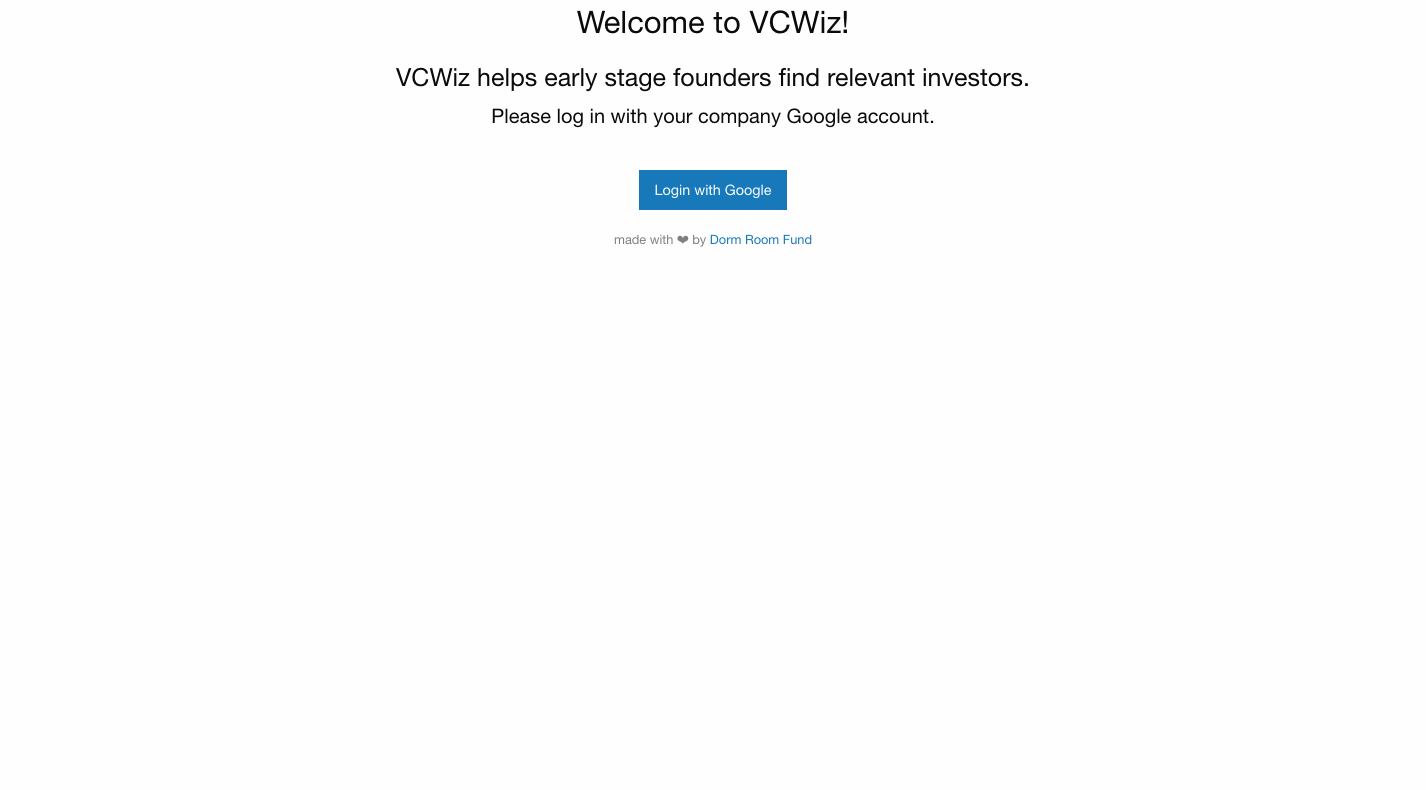
\includegraphics[width=0.9\textwidth]{vcwiz/v1/login.png}
    \caption*{Login Screen}
  \end{minipage}\hfill
  \begin{minipage}{0.33\textwidth}
    \centering
    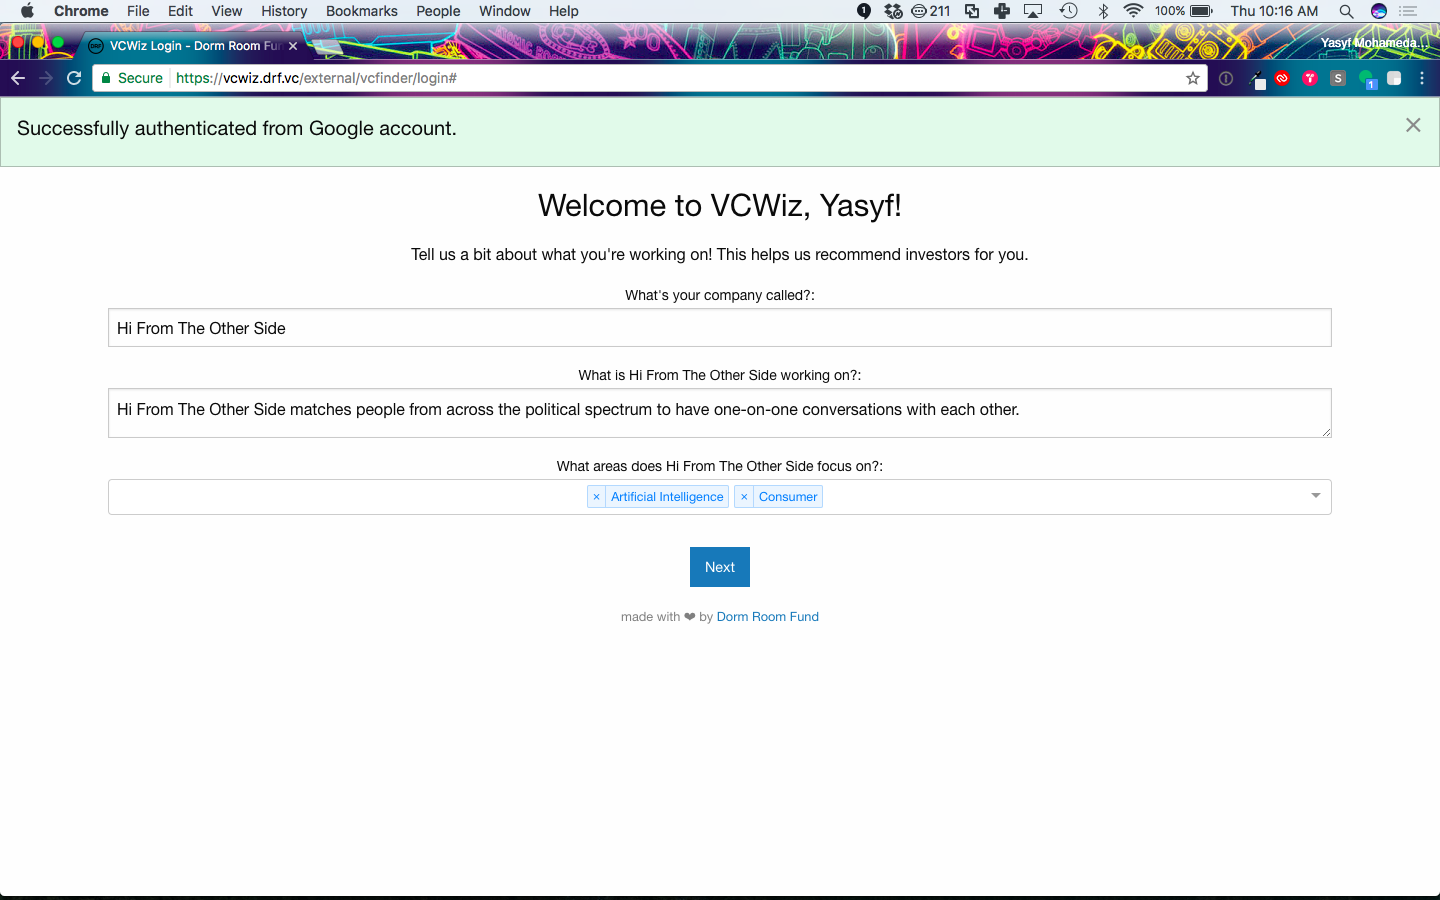
\includegraphics[width=0.9\textwidth]{vcwiz/v1/signup.png}
    \caption*{Signup Screen}
  \end{minipage}\hfill
  \begin{minipage}{0.33\textwidth}
    \centering
    \includegraphics[width=0.9\textwidth]{vcwiz/v1/track.png}
    \caption*{Conversations}
  \end{minipage}
\end{figure}

\subsubsection{Feedback}

We learned a few crucial insights through the launch and test of this first iteration of the application.

With respect to discovery, we realized that founders do not find investors by looking at clusters of similar investors from a few seeds, as our model assumed. Instead, investors were found by examining the previous investors of similar companies to the one in question. While it meant that our kNN-based approach performed poorly for users, it reduced our discovery problem to a version of the very popular Netflix Prize~\cite{netflixpize} problem. Similar users (founders/companies) were positive about similar products (investors). We could now apply an entire body of recommendation-system research to the problem.

With respect to research, the biggest mistake we made was to include only a subset of the information we identified as useful for the founder. As a result, founders would end up leaving the platform to do further research, which was disruptive to their workflow.

With respect to outreach, the first major learning was that it was very difficult to convince founders to trust us with their investor conversations, and that anything we could do to build credibility (for example, auto-filling form fields or leveraging the brands of the venture firms we were working with) vastly increased willingness to share data.

The next big learning was that our users were very familiar with a spreadsheet-based experience (either through Streak or with actual spreadsheets), and that trying to replace it was difficult and unnecessary. A very common piece of feedback was that a ``smart spreadsheet'' would be a far superior interface to the existing card-based workflow.

\subsection{V2}

\subsubsection{Design}

The second version of VCWiz was started in July of 2017. It featured a new recommendation engine, which first asked founders to identify competitors (or similar companies) which are more established. These companies were used to generate recommendations based on a simple algorithm, which takes the set of investors from the identified competitors, filters out the eligible ones, and sorts them based on their relevance, popularity, and whether or not they are featured. The popularity of investor $i$ is calculated based on the number of founders who have added $i$ to their outreach list.

\begin{lstlisting}[frame=single,mathescape=true,language=Ruby,basicstyle=\footnotesize,columns=fullflexible]
def recommendations(founder):
  investors $\gets$ founder.company.competitors.flat_map(c => c.investors)
  eligible $\gets$ investors.filter(i => i.industries $\cap$ founder.company.industries $\neq$ $\emptyset$)
  sorted $\gets$ eligible.sort_by(i => [i.featured, |i.industries $\cap$ founder.company.industries|, i.popularity])
  return sorted
\end{lstlisting}

Another addition to the second version was an augmented spreadsheet interface, which looks and feels like a spreadsheet, but auto-completes information about investors based on a VCWiz investor database. Once sufficient information had been entered on an investor into a row of the sheet to uniquely identify one record in the database, the remaining fields were filled. This gave the founders an experience they were comfortable with, with the power and ease of use they expected to justify switching tools.

In order to build up the VCWiz investor database, we started with a dataset imported from the Crunchbase Data Venture Program, then further augmented it with several additional sources. We will discuss our data pipeline in depth below.

The venture firms in our database are now tagged with the stage of company they invest in, based on the latest fundraising round that has occurred. These categories are defined (and ordered) as such.

\begin{multicols}{2}
\begin{itemize}
  \item Accelerator
  \item Angel
  \item Pre-Seed
  \item Seed
  \item Series A
  \item Series B
  \item Venture
\end{itemize}
\end{multicols}

N.B. These categories are not necessarily mutually exclusive. For example, an accelerator may indeed give a startup their pre-seed round. The category for ``Venture'' captures all growth-stage companies (Series C and later).

Finally, we refined the stages a tracked investor could fall into, based on feedback from founders who were currently fundraising. The list below indicates the ordering over stages that is used throughout the platform.

\begin{multicols}{2}
\begin{itemize}
  \item My Wishlist
  \item Asked for Intro
  \item In Talks
  \item Need to Respond
  \item Pitching
  \item Committed
  \item Passed
  \item Not Interested
\end{itemize}
\end{multicols}

\begin{figure}[ht]
  \centering
  \begin{minipage}{0.45\textwidth}
    \centering
    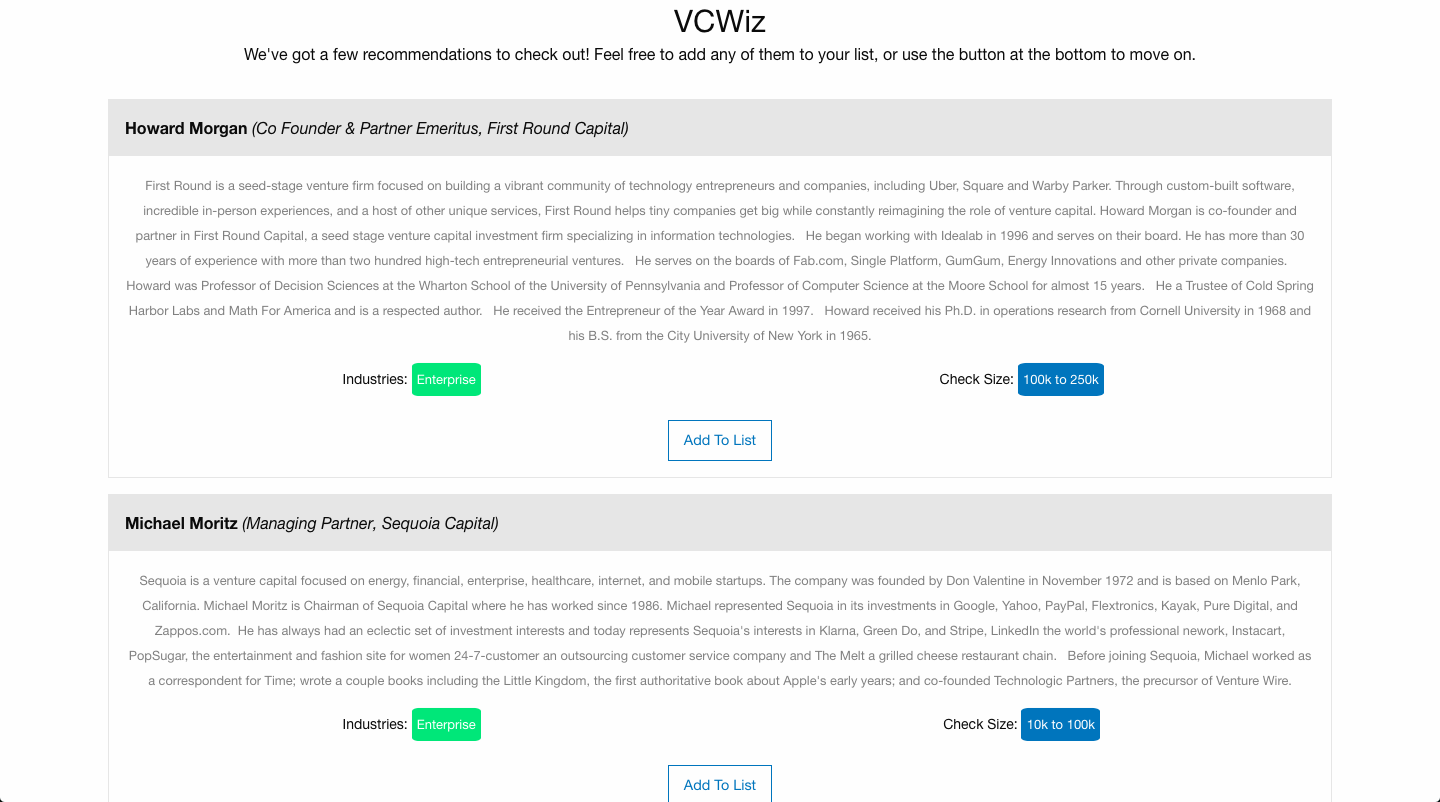
\includegraphics[width=0.9\textwidth]{vcwiz/v2/recommendations.png}
    \caption*{Investor Recommendations}
  \end{minipage}\hfill
  \begin{minipage}{0.45\textwidth}
    \centering
    \includegraphics[width=0.9\textwidth]{vcwiz/v2/track.png}
    \caption*{Conversation Tracker}
  \end{minipage}
\end{figure}

\subsubsection{Feedback}

Following the completion of the second iteration of VCWiz, we did another series of user tests, asking founders to focus specifically on the improvements over the first version.

On discovery, the recommendations were not granular enough, and it was unclear why a certain investor was being recommended. Founders expressed the desire to filter and sift through investors with certain queries (such as some subset of the characteristics being used for recommendations), instead of being blindly handed what appear to be random investors. While there was still a desire for recommendations, it seemed that the place for this was after some amount of filtering, rather than in place of the filtering.

On research, it was felt that the platform still did not provide sufficient information to make it worth using over another tool. Nor did it display the little information it did show in an easy-to-digest way. A common suggestion was to incorporate content from social media and blogging platforms, as investors often use these platforms to demonstrate their interests.

On outreach, the major feedback was that the platform was too rigid. Having pre-defined stages and fields made it difficult to customize the tool for each founder's slightly different workflow, and made them feel like they were fighting the platform, instead of being empowered by it. A common feature request was some way to leverage mutual connections in the outreach.

We used Reichheld's Net Promoter Score (NPS) \cite{reichheld2003one} to track the growth potential of the product with respect to founders. At this stage, the product had an NPS of -50, which is very weak. Only 25\% of founders said they would recommend the product to a friend.

\subsection{V3}

The third iteration of VCWiz was started September of 2017, and aimed to incorporate all the previous feedback. The goal was for the end result to be a production-ready product that launches publicly. The interface and interactions were redesigned from the ground up, this time with the help of a professional designer. The functionality is still split across the three categories of discovery, research, and outreach, though each is now as feature-complete as the competing products which solve a narrower need. We embraced the feedback from founders that the product needed to be comprehensive and holistic, and have improved upon any of the popular features on other platforms.

We will first give an overview of the features of the third and final iteration of the platform, followed by an in-depth analysis of each component.

\subsubsection{Discovery}

VCWiz's initial screen contains an interface to filter and search for investors, by all the characteristics discussed previously, as well as by name and more novel metrics, such as topics often discussed. There are also options to constrain and modify the filters, such as changing a filter from a logical OR to a logical AND. In addition to the filtering and searching, there are curated lists of investors that meet specific criteria, ordered by popularity, and selectively shown to founders based on characteristics of their startup.

\subsubsection{Research}

Clicking through from any of the results in the filter view bring up a research screen which displays comprehensive information on both a firm, as well as every partner at that firm. Every piece of information mentioned in interviews by founders as being useful is included in this view, including but not limited to biographies, social media links, recent investments, press mentions, blog posts and tweets, favorite topics to talk about, industries often invested in, and common co-investors.

\subsubsection{Outreach}

The outreach functionality of VCWiz is embedded in every screen, as well as having a dedicated dashboard.

Every tool for research and discovery has buttons to add investors and firms to the VCWiz Tracker, a CRM which is synced throughout the platform. Founders see a contextual dropdown showing the status of an investor in their pipeline any time they are researching that investor or their peers. The conversations screen is a dashboard which shows a table-like view, containing the information that was previously put in spreadsheets. We used a table to strike the balance between giving founders an interface they were familiar with, and displaying the information in a sufficiently detailed way. The data in this table is populated and updated through an integration with the founder's email provider.

In addition to merely tracking conversations, this version of VCWiz also overlays each screen containing details about an investor with a subset of the founder's email graph, showing them the shortest path(s) to the given investor in their network. This allows the founder to understand how likely they are to be able to reach an investor without a click.

The implementation and launch of this tool is detailed in the following chapter.

Shortly after the public launch of this third version of VCWiz on January 25th, 2018, we surveyed active founders on the platform to again calculate the NPS. This time, we received 117 responses, with an NPS of 0, a significant jump from the last version. 63\% of users agreed that they would recommend VCWiz to a friend, up dramatically from 25\% previously.

\begin{figure}[ht]
  \centering
  \begin{minipage}{0.33\textwidth}
    \centering
    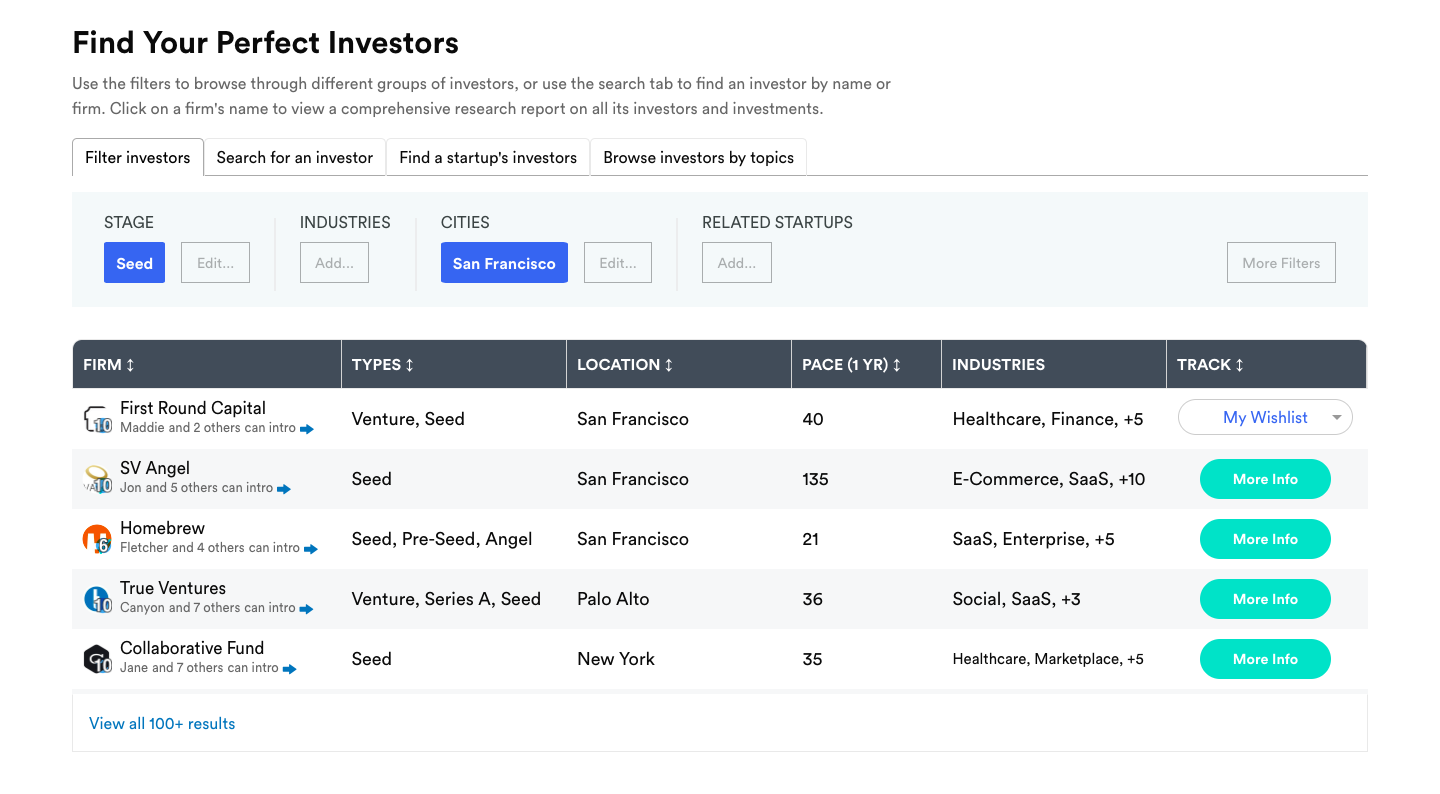
\includegraphics[width=0.9\textwidth]{vcwiz/v3/filter.png}
    \caption*{Filter \& Search}
  \end{minipage}\hfill
  \begin{minipage}{0.33\textwidth}
    \centering
    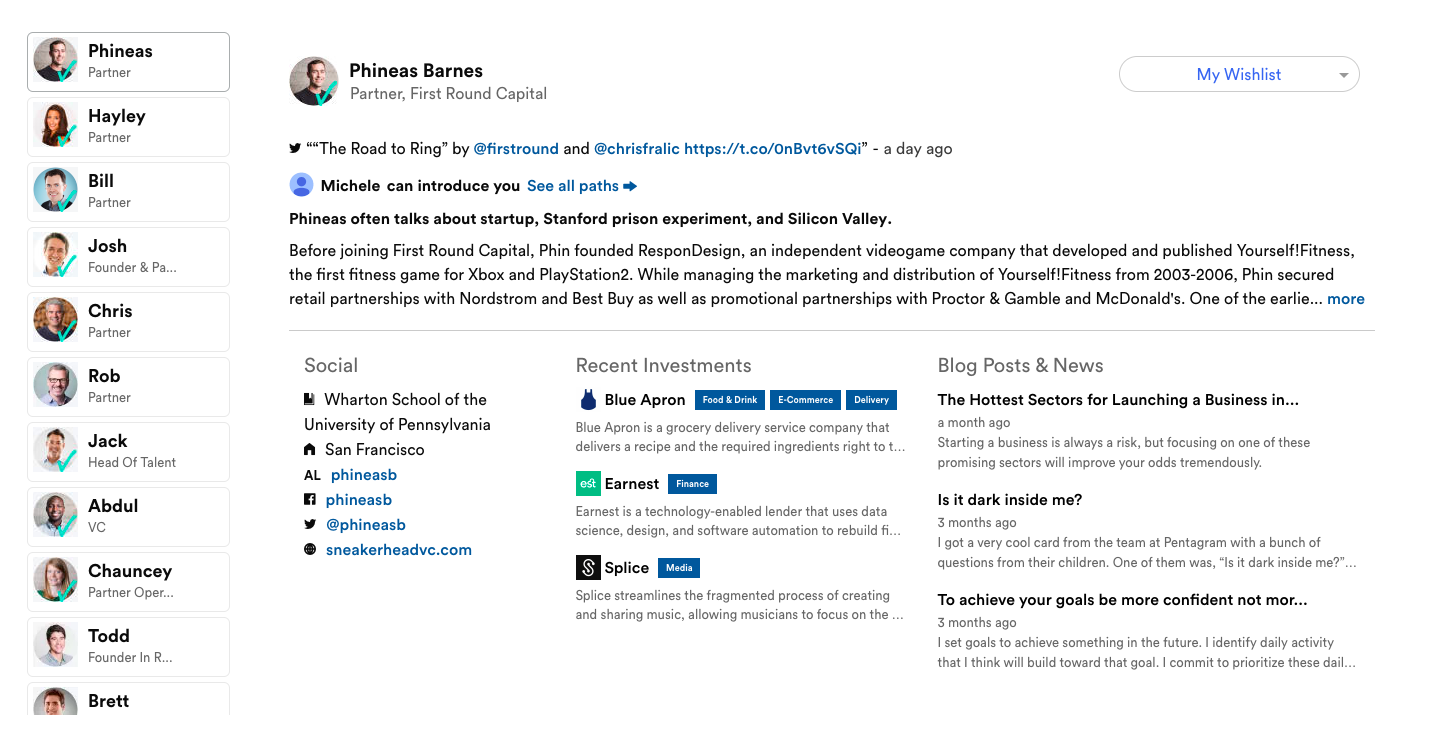
\includegraphics[width=0.9\textwidth]{vcwiz/v3/investor.png}
    \caption*{Investor Research}
  \end{minipage}\hfill
  \begin{minipage}{0.33\textwidth}
    \centering
    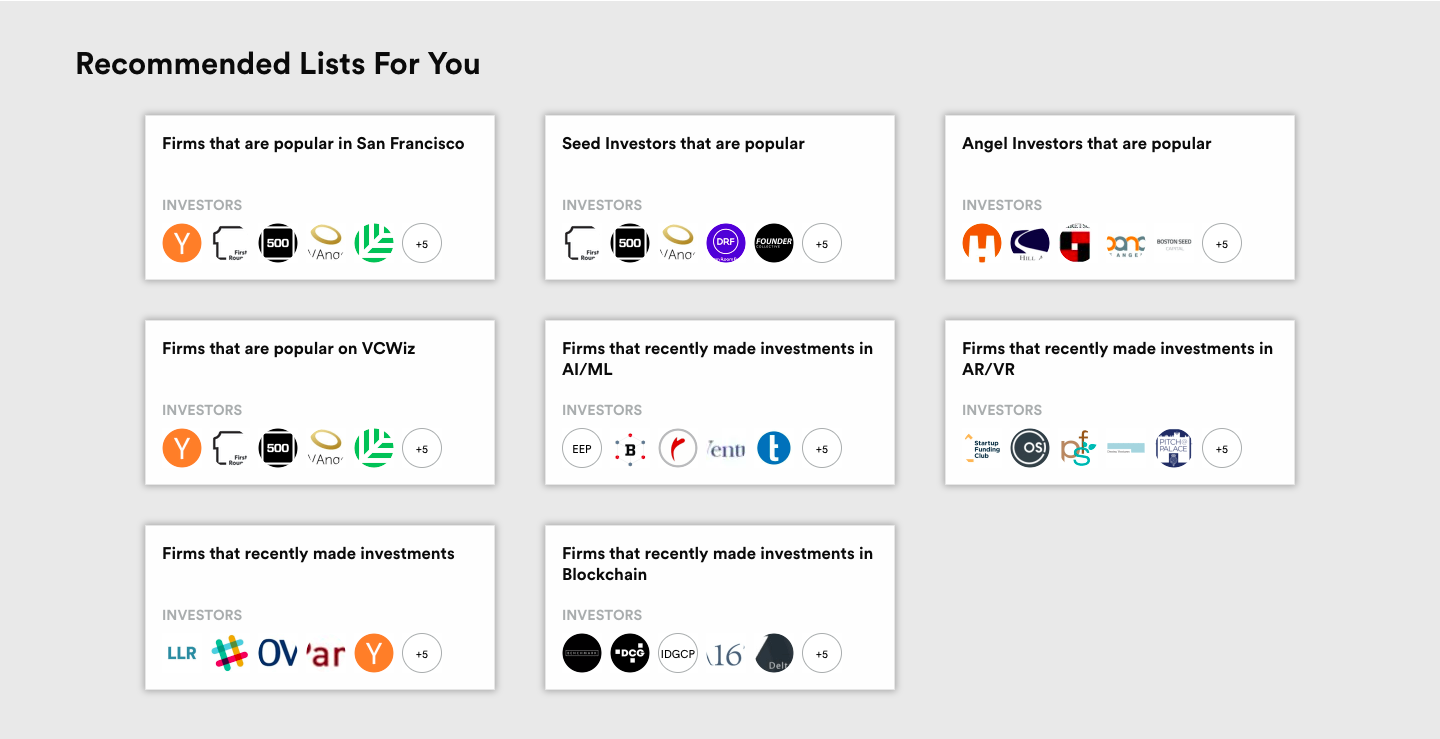
\includegraphics[width=0.9\textwidth]{vcwiz/v3/lists.png}
    \caption*{Curated Firm Lists}
  \end{minipage}
\end{figure}
